\documentclass[11pt]{article}

\usepackage{graphicx}
\usepackage{bm}
\usepackage{siunitx}
\usepackage{booktabs}
\usepackage{xcolor}
\usepackage{authblk}
\usepackage{amsmath}
\usepackage{amssymb}
\usepackage{amsthm}
\usepackage{todonotes}
%\usepackage[normalem]{ulem}
\usepackage{float}
\usepackage{commath}
\usepackage{fancybox}
\usepackage{hyperref}
\usepackage{url}
\usepackage[margin=0.5in]{geometry}
\usepackage[backend=biber, style=authoryear, citestyle=authoryear, autocite=inline, isbn=true]{biblatex} % package for bibliography 
%\DeclareLanguageMapping{english}{english-apa}

\theoremstyle{definition}
\newtheorem{Def}{Definition}[section]
\newtheorem{Eg}{Example}[section]
\newtheorem{Rm}{Remark}[section]
\newtheorem{Ex}{Exercise}[section]
\newtheorem{Prop}[Def]{Proposition}
\newtheorem{Lem}[Def]{Lemma}
\newtheorem{Thm}[Def]{Theorem}
\newtheorem{Cor}[Def]{Corollary}
\newtheorem{Rem}[Def]{Remark}
\newtheorem{Ass}[Def]{Assumption}
\newtheorem{Met}[Def]{Method}
\newtheorem{Res}[Def]{Result}
\newcommand{\red}{\textcolor{red}}
\newcommand{\E}{\mathbb{E}}
\newcommand{\R}{\mathbb{R}}

\addbibresource{sdewind.bib}

%\renewbibmacro*{title}{%
%  \ifboolexpr{
%    test {\iffieldundef{title}}
%    and
%    test {\iffieldundef{subtitle}}
%  }
%    {}
%    {\printtext{%
%     \printtext[titlecase]{\usefield{\uline}{title}}%
%     \setunit{\subtitlepunct}%
%     \printfield[titlecase]{subtitle}}%
%     \newunit}%
%  \printfield{titleaddon}}

\setcounter{page}{1}

\begin{document}

\title{ Stochastic Wind Power Forecasting }  % \\  \small{Report}}

%\author[1]{Waled Alhaddad}
\author[1]{Renzo Caballero}
\author[2]{Ahmed Kebaier}
\author[3]{Marco Scavino}
\author[4]{ Ra\'ul  Tempone}
%\author[2]{Corresponding Author\thanks{email@2nduniversity.com}}
\affil[1,4]{CEMSE Division, King Abdullah University of Science and Technology (KAUST), Saudi Arabia}
\affil[2]{{\color{red}Université Paris 13, Sorbonne Paris Cité, LAGA, CNRS (UMR 7539), Villetaneuse, France}}
\affil[3]{Universidad de la Rep\'ublica, Instituto de Estad\'{\i}stica (IESTA), Montevideo, Uruguay}
\affil[4]{Alexander von Humboldt Professor, RWTH Aachen University, Germany}

%\author{ Waled Alhaddad \textsuperscript{\textasteriskcentered} \qquad Ahmed Kebaier\textsuperscript{\ddag} \qquad Ra\'ul  Tempone\textsuperscript{\textasteriskcentered}\textsuperscript{\textdagger} \\
%\textsuperscript{\textasteriskcentered}CEMSE Division, King Abdullah University of Science and Technology (KAUST), Saudi Arabia \\ \textsuperscript{\textdagger}Alexander von Humboldt Professor, RWTH Aachen University, Germany
% \\ \textsuperscript{\ddag}Université Paris 13, Sorbonne Paris Cité, LAGA, CNRS (UMR 7539), Villetaneuse, France}

\maketitle
%\thispagestyle{empty}

%%%%%%%%% ABSTRACT

\begin{abstract}

Reliable wind power generation forecasting is crucial for applications such as the allocation of energy reserves, optimization for electricity price, and operation scheduling of conventional power plants. We propose a data-driven model based on parametric Stochastic Differential Equations (SDEs) to capture the real asymmetric dynamics of wind power forecast errors. Our SDE framework features time-derivative tracking of the forecast, time-varying mean-reversion parameter, and an improved state-dependent diffusion term. The methodology we developed allows the simulation of future wind power production paths and to obtain sharp empirical confidence bands. All the procedure is agnostic of the forecasting technology and enables comparing different forecast providers. We apply the model to historical Uruguayan wind power production data and forecasts during the period April-December 2019.

\end{abstract}

Keywords: Wind power, probabilistic forecasting, stochastic differential equations, Lamperti transform, 

numerical optimizaton, model selection.

2020 AMS Subject Classification: 60H10, 62M20, 65K10.

%%%%%%%%% BODY TEXT

%---BEGIN SECTION 1---

\section{Introduction}  \label{Section_1}

Despite the Covid-19 pandemic caused ``the biggest shock to the global energy system in more than seven decades'' and the recent report released on April 30, 2020, by the International Energy Agency (\url{https://www.iea.org/reports/global-energy-review-2020}) stresses that projections of energy demand will fall 6\% in 2020 - seven times the decline after the 2008 global financial crisis - it is emphasized that ``renewables are set to be the only energy source that will grow in 2020, with their share of global electricity generation projected to jump thanks to their priority access to grids and low operating cost'' (\cite{IEA}). 

Although the growth of renewables in electricity generation in 2020 is set to be lower than in previous years,  solar PV and wind are on track to help lift renewable electricity generation by 5\% in 2020, aided by higher output from hydropower. \\

Wind and solar energy are expanding renewable generation capacity, experiencing record growth in the last years.

\begin{figure}[H]
\centering
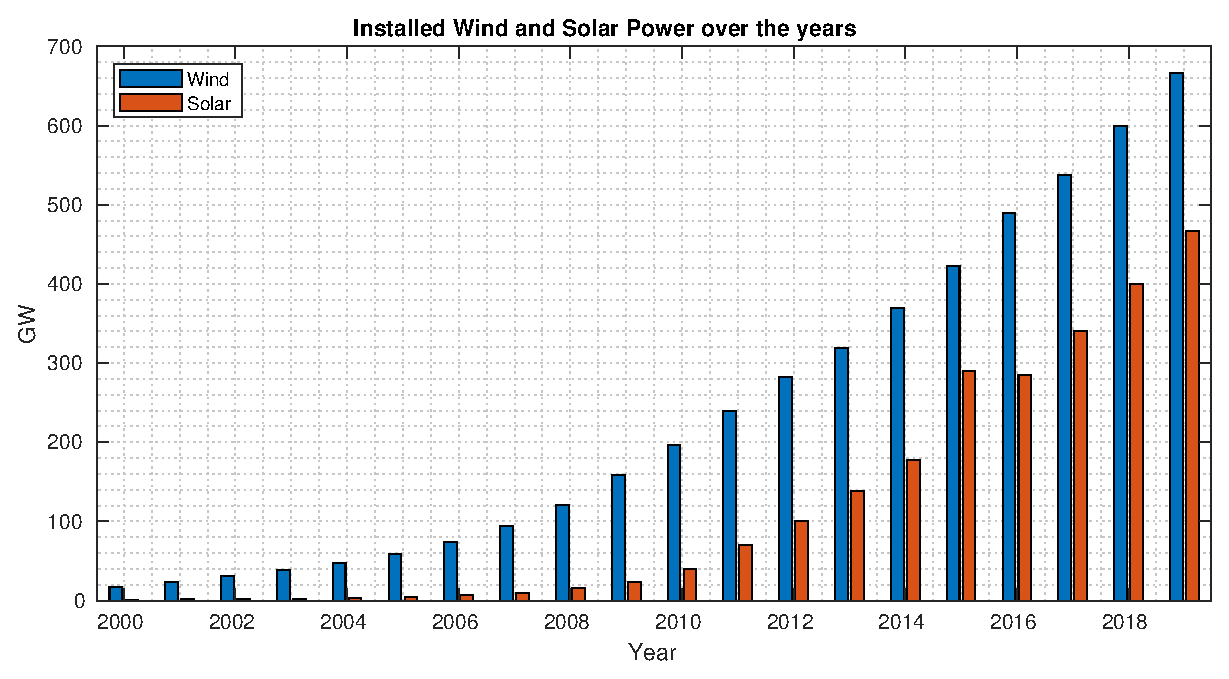
\includegraphics[width=0.9\textwidth]{plots/wind_and_solar/plot_over_years.eps}
\caption{Installed wind and solar power over the years \cite{sultana2017review}. We recall the importance of accurate forecasts to use green energies optimally.}
\end{figure}

Reliable wind power generation forecasting is crucial for the following applications (see, for example, \cite[5]{gieb}, \cite[162]{chang}, \cite{zhbo}):
\begin{itemize}
\item Allocation of energy reserves such as water levels in dams or oil, and gas reserves.
\item Operation scheduling of controlable power plants.
\item Optimization of the price of electricity for different parties such as electric utilities, Transmission system operator (TSOs), Electricity service providers (ESPs), Independent power producers (IPPs), and energy traders.
\item Maintenance planning such as that of power plants components and transmission lines.

\end{itemize}

Different methods have been applied to wind power forecasting. They can be generally categorized as follows: physical models, statistical methods, artificial intelligence methods, and hybrid approaches. The output of such methods is usually a deterministic forecast. Occasionally probabilistic forecasts are produced through uncertainty propagation in the data, parameters, or forecast ensembles. {\color{red} Expand discussion about works on probabilistic forecasting.} However, there is a lack of simulating and producing data-driven stochastic forecasts based on forecasting models. It is crucial to capture the forecast's actual performance as it has been known that different forecasting technologies exhibit different behavior for different wind farms and seasons (\cite{chang}). This is due to many factors that forecast are challenged to capture, such as the surrounding terrains of the wind farm and the condition of the blades such as icing, wear and tear, or dirt. It is known that complex terrains in both off shore and on shore locations decrease the accuracy of wind power forecasts significantly (\cite{schicker2017short}). It also has been shown that the performance of forecasts varies from month to month. Thus the performance of wind power forecasts is location and time dependent.

Many approaches have been taken to evaluate the uncertainty of a given forecast. There are two types of errors: level errors and phase errors. The use of mean or median errors in this context may be misleading as wind power forecast errors are asymmetric. This is a natural consequence of wind power being non-negative and bounded by the maximum capacity of production. This is important as the associated cost to power forecast errors is also asymmetric due to different costs for up and down power regulations, which are determined by the electricity market (\cite{tsitsiklis2015pricing}).

We propose to model wind power forecast errors using parametric stochastic differential equations (SDEs) whose solution defines a stochastic process. This resultant stochastic process describes the time evolution dynamics of wind power forecast errors while capturing properties such as a correlation structure and the inherent asymmetry. Additionally, the model we propose is agnostic of the forecasting technology and serves to complement forecasting procedures by providing a data-driven stochastic forecast. Hence, we can evaluate wind power forecasts according to their real-world performance, and we can compare different forecasting technologies. Most notably, we can simulate future wind power production given a deterministic wind power forecast. Future wind power production using Monte Carlo methods, as well as the analytic form of the proposed SDE, can be used in optimal control problems involving wind power production.

Previous attempt by (\cite{mozuma}) considered stochastic wind power forecast models based on stochastic differential equations. Here, we propose an improved model featuring time derivative tracking of the forecast, time-dependent mean reversion, modified diffusion, and non-Gaussian approximations. We apply the model to Uruguayan wind power forecasts together with historical wind power production data pertaining to the year 2019. \\

The rest of the paper is organized as follows. In Section \ref{Section_2}, we introduce the main characteristics of a real data set encompassing the normalized wind power production in Uruguay during the period April-December 2019, joint with the most accurate predictions, as highlighted in our posterior analysis, performed by one out of the three sources of forecast providers. The significant steps for constructing phenomenological models of the normalized wind power production and the forecast error based on stochastic differential equations are described in Section \ref{Section_3}. The application of the Lamperti transform with unknown parameters in Section \ref{Section_4} leads to model the forecast error through a stochastic differential equation with a unit diffusion coefficient. In Section \ref{Section_5}, we write down the expressions for the likelihood functions of the forecast error in its original space and the Lamperti space. We also derive simple approximations of the likelihood functions. Section \ref{Section_5} concludes with the description of the optimization algorithm to compute approximate maximum likelihood estimates, including the case where we expand the model comprising an initial transition from the time the forecast is performed to the time of the first forecast.

In Section \ref{Section_6}, we apply our proposed numerical estimation procedures to the Uruguay wind and forecast dataset, comparing two alternative models and assessing, for the best candidate model, the performance of three different forecast providers. Section \ref{Section_7} concludes the paper. 
The proofs of the existence, strong uniqueness, and boundedness of the SDE solutions used to model normalized wind power production and its forecast error are given in the Appendix.

%---END SECTION 1---

%---BEGIN SECTION 2---

\section{Wind power production data in Uruguay and forecast providers } \label{Section_2}

In recent years, Uruguay has triggered a remarkable change in its energy matrix. In (\cite{irena}, p.23), Uruguay is among those countries showcasing innovation, like Denmark, Ireland, Germany, Portugal, and Spain, with proven feasibility of managing annual variable renewable energy (VRE) higher than 25\% in power systems. 

According to (\cite{ren21}, pp.118-119), in 2018, Uruguay achieved 36\% of its electricity production from variable wind energy and solar PV, raising the share of generation from wind energy more than five-fold in just four years, from 6.2\% in 2014 to 33\% in 2018. 

At present, Uruguay is fostering even higher levels of wind penetration by boosting regional power trading with Argentina and Brazil. 
In this rapidly evolving scenario, it is essential to analyze national data on wind power production joint with wind power short-term forecastings to orientate and assess the strategies and decisions of wind energy actors and businesses. 

Our study is based on publicly available data (source: Administrator of Electric Market) on the wind power production in Uruguay for the period April-December 2019, that we adequately normalized with respect to the present $\SI{1474}{\mega\watt}$ maximum installed wind power capacity. Each day, wind power production recordings are available every ten minutes.  In this work, we have also considered data from three different forecast providers, available each day starting at 1 pm.

The next Figure \ref{fig:sample_data} shows the wind power real production during four segments 24-hour long selected from the observation period together with their corresponding hourly short-term forecast, computed by a forecast provider. For the sake of visualization clarity, this Section relies only on forecasts from one provider, called "provider A" from now on, ranked as the most accurate forecast provider, as it emerged from our posterior analysis.

\begin{figure}[H]
\centering
\includegraphics[width=0.45\textwidth]{plots/four_days/377.eps}
\includegraphics[width=0.45\textwidth]{plots/four_days/417.eps}\\
\quad\\
\includegraphics[width=0.45\textwidth]{plots/four_days/437.eps}
\includegraphics[width=0.45\textwidth]{plots/four_days/477.eps}
\caption{Four 24-hour segments with the wind power real production in Uruguay (orange line) recorded every ten minutes, and the hourly wind power production forecasted by provider A (blue line).}
  \label{fig:sample_data}
\end{figure}

A view of the global discrepancy between the real production and the forecasted production, during the nine months observation period, is summarized through the forecast error histograms in Figure \ref{fig:data_curtailing}, where we also partitioned the forecast errors according to three contiguous categories of normalized generated power. Low normalized generated power corresponds to the range $[0,0.3]$, mid-power refers to the range $]0.3,0.6]$, and high-power to the range $]0.6,1]$.

\begin{figure}[H]
\centering
\includegraphics[width=0.45\textwidth]{plots/LP_6.eps}
\includegraphics[width=0.45\textwidth]{plots/MP_6.eps}\\
\quad\\
\includegraphics[width=0.45\textwidth]{plots/HP_6.eps}
\includegraphics[width=0.45\textwidth]{plots/AP_6.eps}
\caption{Wind production forecast error histograms during the period April-December 2019: low-power (upper-left plot), mid-power (upper-right plot), high-power (lower-left plot), and the global range of power (lower-right plot).}
  \label{fig:data_curtailing}
\end{figure}

We may observe that all the histograms in Figure \ref{fig:data_curtailing} exhibit skewed patterns, to a different extent, as well as extreme observations. The presence of these features can be partly explained. The data analysis highlighted that, during several 24-hour segments, the system operators decided to reduce or even cease the wind power production. Indeed, as recalled in (\cite{irena2}, p.3), ``Uruguay experiences high curtailment levels because generation exceeds demand.'' Despite the large country's interconnection capacity with Argentina and Brazil, there is no active cross-border market; the energy is traded via ad hoc short-term agreements. ``Even with interconnection capacity exceeding peak demand, the power system experiences high VRE curtailment, mostly at night when wind generation exceeds demand.''
  
The curtailment of the wind power production imposed by the system operators has a strong influence on the forecast error. To build a model that, driven by the available forecast, allows the inclusion of true power production with a prescribed degree of uncertainty, it is necessary to remove the data segments affected by wind curtailment.

Once we removed all the 24-hour segments showing wind curtailment, we set up a dataset containing 147 daily segments. 
In the absence of the curtailment intervention, the forecast error histograms are shown below in Figure \ref{fig:data_after_clean}, where it can be appreciated skewness reduction, except for low power forecast errors histogram.

\begin{figure}[H]
\centering
\includegraphics[width=0.45\textwidth]{plots/LP.eps}
\includegraphics[width=0.45\textwidth]{plots/MP.eps}\\
\quad\\
\includegraphics[width=0.45\textwidth]{plots/HP.eps}
\includegraphics[width=0.45\textwidth]{plots/AP.eps}
\caption{Wind production forecast error histograms during the period April-December 2019 after removing 24-hour segments with artificial wind curtailment: low-power (upper-left plot), mid-power (upper-right plot), high-power (lower-left plot), and the global range of power (lower-right plot).}
  \label{fig:data_after_clean}
\end{figure}

In this stage of data preprocessing, we obtain another useful result by applying the first-order difference operator to the forecast errors. 
The forecast error transition histograms, displayed in the next Figure \ref{fig:error_transitions}, will constitute later a reference for the visual assessment of the global fit of the proposed models.

\begin{figure}[H]
\centering
\includegraphics[width=0.45\textwidth]{plots/LP_t.eps}
\includegraphics[width=0.45\textwidth]{plots/MP_t.eps}\\
\quad\\
\includegraphics[width=0.45\textwidth]{plots/HP_t.eps}
\includegraphics[width=0.45\textwidth]{plots/AP_t.eps}
\caption{Forecast error transition histograms during the period April-December 2019 without wind power production curtailment: low-power (upper-left plot), mid-power (upper-right plot), high-power (lower-left plot), and the global range of power (lower-right plot).}
\label{fig:error_transitions}
\end{figure}

The histograms in Figure \ref{fig:error_transitions} feature a non-Gaussianity trait and provide initial input for the model-building stage, which is described in Section next.
Later, in Section \ref{Section_4}, guided from inferring the unknown model parameters, we will also propose transforming data as a strategy that naturally leads to an alternative model.

%---END SECTION 2---

%---BEGIN SECTION 3---

\section{Phenomenological  Model} \label{Section_3}

After analyzing the available dataset, we are now in the condition to build a type of phenomenological model for the normalized wind power generation forecasts that, in its most general form, is a stochastic process $X = \{X_t, \, t \in [0, T] \}$  defined by the following stochastic differential equation (SDE):

\begin{equation}
\begin{cases}
    \dif X_t &=  a(X_t; p_t, \dot{p}_t,\bm{\theta})\dif t + b (X_t; p_t, \dot{p}_t, \bm{\theta} )\dif W_t, \quad t \in [0,T]  \\
     X_0  &=  x_0 \in [0,1],
\end{cases}
 \label{eq:main}
\end{equation} 

where

\begin{itemize}
\item $a(\cdot; p_t, \dot{p}_t, \bm{\theta}): [0,1] \to \mathbb{R} $  denotes a drift function,
\item $b(\cdot; p_t, \dot{p}_t, \bm{\theta}): [0,1] \to \mathbb{R}^+ $  a  diffusion function,
\item $\bm{\theta}$ is a vector of unknown parameters,
\item $(p_t)_{t \in [0,T]}$ is a time-dependent deterministic function $[0,1]$-valued and $ (\dot{p}_t)_{t \in [0,T]}$ is its time derivative,
\item $\{W_t, \, t \in [0,T] \}$ is a standard real-valued Wiener process.
\end{itemize}

In this work, $(p_t)_{t \in [0,T]}$ is to be considered as a deterministic forecast for the normalized wind power generation, which is provided by an official source. 

Our goal is to achieve a specification of the model (\ref{eq:main}) to follow the available normalized wind power forecasts closely while ensuring its unbiasedness with respect to the forecast.

\subsection{Physical Constraints} \label{Physical_Constraints}

Let $(p_t)_{t \in [0,T]}$ be the available prediction function for the normalized wind power, which is an input to this approach. To start with the model specification, first, we introduce a time-dependent drift function that features the mean-reverting property as well as derivative tracking:\begin{equation}
a(X_t; p_t, \dot{p}_t, \bm{\theta}) = \dot{p}_t  - \theta_t (X_t - p_t),  \label{drift:meanrev-derivtrack}
\end{equation} 
where $ (\theta_t)_{t \in [0,T]} $ is a positive deterministic function, whose range depends on $\bm{\theta}$, as will be explained shortly.

Now, looking at the normalized wind power generation forecast process $X_t$, modeled as solution to the It\^{o} stochastic differential equation (\ref{eq:main}) with the drift specified in (\ref{drift:meanrev-derivtrack}), it is straightforward to check that $\mathbb{E} \left[X_t\right] = p_t$, given $  \mathbb{E}\left[X_0\right] = p_0$. The application of  It\^{o}'s lemma % on $g(X_t, t) = X_t e^{\int_{0}^{t} \theta_s \dif s}$, leads to 
leads to
%\begin{equation*}
%\dif \left( X_t e^{\int_{0}^{t} \theta_s \dif s} \right) = e^{\int_{0}^{t} \theta_s \dif s} (\dot{p}_t + \theta_t p_t ) \dif t  + e^{\int_{0}^{t} \theta_s \dif s}b (X_t; p_t, \dot{p}_t, \bm{\theta} ) \dif W_t,
%\end{equation*}
%whose integral form is
\begin{equation}
e^{\int_{0}^{t} \theta_s \dif s}  X_t - X_0 = \int_{0}^{t}  (\dot{p}_s + \theta_s p_s ) e^{\int_{0}^{s} \theta_u \dif u} \dif s + \int_{0}^{t}  b (X_s; p_s, \dot{p}_s, \bm{\theta} )  e^{\int_{0}^{s} \theta_u \dif u}\dif  W_s.   \label{eq:tomeanX}
\end{equation} 
Taking expectation on (\ref{eq:tomeanX}) we obtain
%\begin{align}
%\mathbb{E} \left[X_t\right] & = e^{ - \int_{0}^{t} \theta_s \dif s} \left(  \mathbb{E} \left[X_0\right] +   \int_{0}^{t}  (\dot{p}_s + \theta_s p_s ) e^{\int_{0}^{s} \theta_u \dif u} \dif s   \right) \nonumber \\ 
%& =  e^{ - \int_{0}^{t} \theta_s \dif s} \left(  \mathbb{E} \left[X_0\right] +   \int_{0}^{t}  \dot{p}_s e^{\int_{0}^{s} \theta_u \dif u} \dif s +  \big[ p_s \, e^{\int_{0}^{s} \theta_u \dif u} \big]^{t}_0  - \int_{0}^{t}  \dot{p}_s e^{\int_{0}^{s} \theta_u \dif u} \dif s  \right) \nonumber \\
%& =  e^{ - \int_{0}^{t} \theta_s \dif s} \left(  \mathbb{E}\left[ X_0\right] + p_t \, e^{ \int_{0}^{t} \theta_s \dif s} - p_0 \right) = p_t. \label{eq:meanX}
%\end{align}
\begin{equation}
\mathbb{E} \left[X_t\right] =  e^{ - \int_{0}^{t} \theta_s \dif s} \left(  \mathbb{E}\left[ X_0\right] + p_t \, e^{ \int_{0}^{t} \theta_s \dif s} - p_0 \right) = p_t.
\label{eq:meanX}
\end{equation}

 At this stage, the process defined by (\ref{eq:main}) with drift (\ref{drift:meanrev-derivtrack}) satisfies the two following properties: 
\begin{itemize}
\item it reverts to its mean $p_t$, with a time-varying speed $ \theta_t$ that is proportional to the deviation of the process $X_t$ from its mean,
\item it tracks the time derivative $\dot{p}_t$.  
\end{itemize} 

Remark: Observe that a mean-reverting model without derivative tracking shows a delayed path behavior. For instance, consider the diffusion model (\ref{eq:main}) with $a(X_t; p_t, \bm{\theta}) = - \theta_0 (X_t - p_t)\,, \theta_0 > 0$. In this case, given  $ \mathbb{E} \left[X_0\right] = p_0$, the diffusion has mean $\mathbb{E} \left[X_t\right] = p_t - e^{- \theta_0 t } \int_0^t \dot{p}_s  e^{\theta_0 s} \dif s$. The next Figure (\ref{fig:derivative_tracking}) illustrates how different behave the estimated confidence bands for two diffusion models with and without derivative tracking, fitting the same daily segment.

\begin{figure}[H]
\centering
  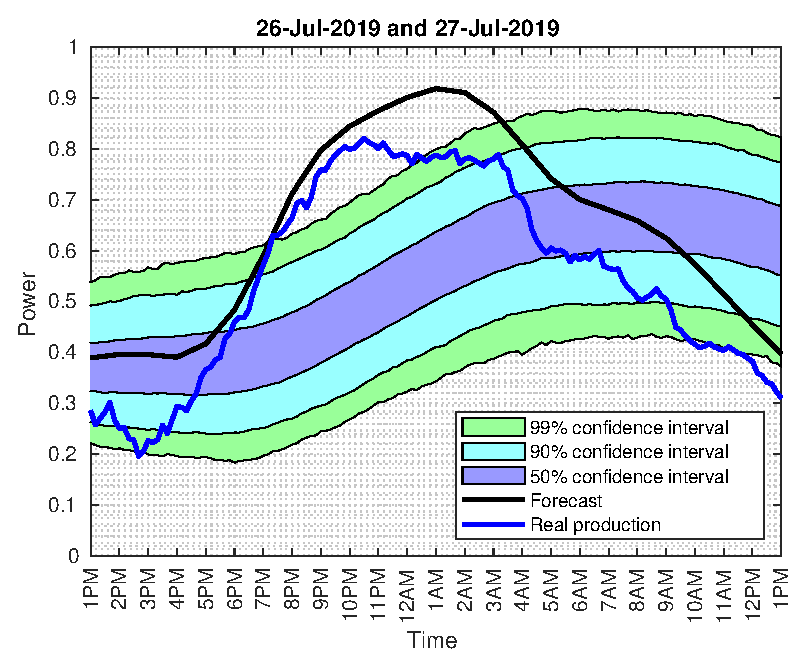
\includegraphics[width=0.45\textwidth]{plots/31.eps}\includegraphics[width=0.45\textwidth]{plots/31_2.eps}
  \caption{Pointwise confidence bands fitted, for the same daily segment, through diffusion models without derivative tracking (plot on the left) and with derivative tracking (plot on the right).}
  \label{fig:derivative_tracking}
\end{figure}

The forecast and production wind power data of Uruguay are normalized with respect to the installed power capacity during the period of observation. Thus, the mean-reverting level lies in $[0,1]$, and the process $X_t$  must take values in the same interval, a requirement that is not automatically fulfilled through the derivative tracking. To impose that the state space of $X_t$ is $[0,1]$, we may choose a convenient diffusion term, and require that the time-varying parameter $ \theta_t$ satisfies an ad-hoc condition.
 
Let $\bm{\theta} = (\theta_0,\alpha)$, and choose a state-dependent diffusion term that avoids the process exiting from the range $[0,1]$ as follows:
  \begin{equation}
    b (X_t; \bm{\theta} )= \sqrt{2 \alpha \theta_0 X_t (1 - X_t)}
  \end{equation}
  where $\alpha >0$ is an unknown parameter that controls the path variability. This diffusion term belongs to the Pearson diffusion family and, in particular, it defines a Jacobi type diffusion. It is useful to recall that (\cite[440]{foso}) a Pearson diffusion is a stationary solution to a stochastic differential equation of the form \begin{equation}
    \dif X_t = - \theta (X_t - \mu)\dif t + \sqrt{2 \theta \left(a X_t^2 + b X_t + c\right)} \dif W_t
    \label{eq:poly_diff}
  \end{equation}
where $\theta>0$, and $a$, $b$, and $c$ are parameters such that the square root is well defined when $X_t$ is in the state space. These parameters, together with $\mu$, the mean of the invariant distribution, determine the state space of the diffusion as well as the shape of the invariant distribution.

An exhaustive classification of the (stationary) Pearson diffusions is presented in (\cite[440-443]{foso}) where, in particular, it is discussed the case $a < 0$ and $b(x; \bm{\theta}) = \sqrt{2 a \theta x (x-1)}$, where the invariant distribution is a Beta distribution with parameters $\left( \frac{\mu}{-a}, \frac{1 - \mu}{-a} \right),$ that leads to the well-known Jacobi diffusions, so-called because the eigenfunctions of the infinitesimal generator of these processes are the Jacobi polynomials (see, for example, \cite[2860-2861]{leph}). 

It is worth mentioning that Jacobi diffusions have been successfully applied in several disciplines, among them finance (see \cite{vago} and references therein) and neuroscience (\cite{dotala}).

However, a distinctive feature in our proposed model 
\begin{equation}
\begin{cases}
    \dif X_t&= \left(\dot{p}_t  - \theta_t (X_t - p_t) \right) \dif t +\sqrt{2 \alpha \theta_0 X_t (1 - X_t)} \dif W_t, \quad t \in [0,T]  \\
   X_0 &=  x_0\in [0,1] ,
\end{cases}
\label{ourmodel}
\end{equation}

is that the drift term contains the time-varying parameter $\theta_t$, rendering the solution $X_t$ of (\ref{ourmodel}) to a non-stationary and time-inhomogeneous process. To ensure that the process $X_t$ is the unique strong solution of (\ref{ourmodel}) for all $t \in [0,T]$ with state space $[0,1]$ a.s., the mean-reversion time-varying parameter must satisfy the condition:

\begin{equation}
\theta_t\geq \max\left(\frac{\alpha\theta_0+\dot p_t}{1-p_t},\frac{\alpha\theta_0-\dot p_t}{p_t}\right)\tag{B}. 
\end{equation} \label{condB}
The proof of this theoretical statement is presented in Section \ref{Appendix}. \\

Remark: Condition (B) shows that the time-varying parameter $\theta_t$ becomes unbounded when $p_t = 0$ or $p_t = 1$. Therefore, we consider the following truncated prediction function
\begin{equation}
  p_t^{\epsilon} = \left\{
  \begin{array}{@{}cl@{}}
    \epsilon \!\!\!&\text{if \quad} p_t  < \epsilon  \\
    p_t  \!\!\!&\text{if \quad}  \epsilon \leq p_t < 1 - \epsilon \\
    1 - \epsilon  \!\!\!&\text{if \quad}  p_t \geq 1 - \epsilon
 \end{array}\right.  \label{corrforecast}
\end{equation}
that satisfies $p_t^{\epsilon} \in [\epsilon, 1 - \epsilon]$ for any $0 < \epsilon < \frac{1}{2}$ and $t \in [0,T]$, providing that $\theta_t$ is bounded for every $t \in [0,T]$. \\

Remark: In this work, the analysis of the three different forecast datasets shows that there exists, for any forecast provider, a small $\epsilon >0$ to define the truncated prediction function fulfilling the above condition. \\

From now on, we will keep the notation $p_t$ to denote the truncated prediction function (\ref{corrforecast}), unless specified otherwise. 

\subsection{A model specification for the forecast error}
 After applying to (\ref{ourmodel}) the simple change of variables $$V_t = X_t - p_t \,,$$ we may introduce the following model for the forecast error of the normalized wind power production: 

\begin{equation}
\begin{cases}
\dif V_t&=  - \theta_t V_t\dif t + \sqrt{2 \alpha \theta_0 (V_t +p_t ) (1-V_t-p_t)}\dif W_t, \quad t \in [0,T]  \\
V_0&=  v_0\in [-1 + p_0,1 - p_0].
\end{cases}  \label{VtSDE}
\end{equation}

%---END SECTION 3---

%---BEGIN SECTION 4---

\section{State independent diffusion term: Lamperti transform} \label{Section_4}

Our model (\ref{VtSDE}) for the forecast error has a diffusion term that depends on the state variable $V_t$. Under the conditions that permit to use It\^{o}'s formula on a well-chosen transformation of the process $V$, John Lamperti (\cite{lamp}) first showed that the transformed process is again a diffusion that is solution to a SDE with unit coefficient for the diffusion term. 
A vast literature refers nowadays to this result as the so-called Lamperti transform (see, for example, \cite[40--41]{iacus1}, \cite{moma}, \cite[199--203]{pani}, \cite[98--100]{saso}), which is a basic tool to obtain a SDE for the transformed process whose diffusion term does not depend anymore on the state variable. A remarkable effect of removing the state dependency from the random noise term is to increase the numerical stability of the simulated paths of the transformed process. 
For this reason, some estimation methods of the unknown parameters of non-linear SDE models incorporated the Lamperti's change of variable as part of a more complex approximation procedure (for example, in the case of one-dimensional diffusions, the local linearization method in  \cite{shoz}, or the expansion method in \cite{ait}, later extended to time-inhomogeneous SDEs in \cite{eglix}).
% later extended to multivariate diffusion in \cite{ait2}).

We consider the following Lamperti transform with unknown parameters
%{\color{red} (Remind that continuous-time models with different diffusion term are singular and the likelihood cannot be written down. Besides, it can be unstable to work with low frequency. If the frequency of the data is too low, the Lamperti transform helps to detect this problem (in principle, it is not clear how to determine the right frequency for estimation. )}
%\begin{equation}
%Z_t = h(V_t, t) = \frac{1}{\sqrt{2 \theta_0 \alpha}} \int_{\xi}^{x} \frac{1}{\sqrt{(u + p_t)(1 - u - p_t)}} \,du \Bigg{\vert}_{x = V_t} \,,
%\end{equation}
%where $\xi$ is an arbitrary point of the state space of the process $V$. The choice of $\xi = \frac{1}{2} - p_t$, where $p_t$ is a known input, 
\begin{align}
Z_t = h(V_t, t; \bm{\theta} )  & = \frac{1}{\sqrt{2 \alpha \theta_0 }} \int \frac{1}{\sqrt{(v + p_t)(1 - v - p_t)}} \dif v \Bigg{\vert}_{v = V_t}   = - \sqrt{ \frac{2}{ \alpha \theta_0 }} \arcsin (\sqrt{ 1 - V_t - p_t}) \label{eq:LampZ}
\end{align}
that, after applying It\^{o}'s formula on $h(V_t, t; \bm{\theta} )$, leads to the following SDE with state independent unit diffusion term
\begin{align}
\dif Z_t = \Bigg[  & \frac{\dot{p}_t}{ \sqrt{2 \alpha \theta_0 (V_t + p_t)(1 - V_t - p_t)}}  + \frac{- \theta_t V_t}{ \sqrt{2  \alpha \theta_0 (V_t + p_t)(1 - V_t - p_t)}} - \frac{1}{4} \frac{\sqrt{2 \alpha \theta_0} \left( 1 - 2 (V_t + p_t)\right)}{\sqrt{(V_t + p_t)(1 - V_t - p_t)}}  \Bigg] \dif t + \dif W_t \,. \label{eq:stindepSDE}
\end{align}
After replacing $V_t = 1 - p_t - \sin^2 \left(- \sqrt{ \frac{ \alpha \theta_0}{2} } Z_t \right) $ in (\ref{eq:stindepSDE}), we obtain that the  process $Z_t$ satisfies the SDE
\begin{align}
\dif Z_t & = \left[ \frac{ \dot{p}_t  - \theta_t  \left(1 - p_t - \sin^2 \Big(- \sqrt{ \frac{ \alpha \theta_0}{2} } Z_t \Big) \right) }{\sqrt{2 \alpha \theta_0} \cos\Big(- \sqrt{ \frac{ \alpha \theta_0}{2} } Z_t \Big)  \sin\Big(- \sqrt{ \frac{ \alpha \theta_0}{2} } Z_t \Big)}   - \frac{1}{4}  \frac{\sqrt{2 \alpha \theta_0} \left(1 - 2 \cos^2 \Big(- \sqrt{ \frac{ \alpha \theta_0}{2} } Z_t \Big) \right) }{\cos\Big(- \sqrt{ \frac{ \alpha \theta_0}{2} } Z_t \Big)  \sin\Big(- \sqrt{ \frac{ \alpha \theta_0}{2} } Z_t \Big)} \right]\dif t + \dif W_t \nonumber \\
&  = \left[  \frac{  2  \dot{p}_t - \theta_t (1 - 2 p_t)  + (\alpha \theta_0 - \theta_t) \cos(- \sqrt{2 \alpha \theta_0 } Z_t) }{\sqrt{2 \alpha \theta_0} \sin{(- \sqrt{2 \alpha \theta_0} Z_t)}}  \right] \dif t + \dif W_t.  \label{eq:stindepSDE2}
\end{align}

To summarize the effect of the Lamperti transform visually, we can see in the next Figure (\ref{fig:LP_transitions}) how the forecast error transition histograms (without curtailment) modify in comparison with Figure (\ref{fig:error_transitions}).

In this case, the Lamperti transform has been applied using the optimal estimates of the parameters in the SDE model (\ref{VtSDE}), obtained applying our numerical procedure detailed later in Subsection \ref{opt_sec}.  

\begin{figure}[H]
\centering
\includegraphics[width=0.45\textwidth]{plots/LP_t_LP.eps}
\includegraphics[width=0.45\textwidth]{plots/MP_t_LP.eps}\\
\quad\\
\includegraphics[width=0.45\textwidth]{plots/HP_t_LP.eps}
\includegraphics[width=0.45\textwidth]{plots/AP_t_LP.eps}
\caption{Lamperti transformed forecast error transition histograms during the period April-December 2019 without wind power production curtailment: low-power (upper-left plot), mid-power (upper-right plot), high-power (lower-left plot), and the global range of power (lower-right plot).}
  \label{fig:LP_transitions}
\end{figure}

The shape of the forecast error transition histograms after applying the Lamperti transform has much resemblance with a Gaussian distribution, motivating toward the use of Gaussian-like approximations of the unknown density transition functions of the process $Z_t$.

{\color{red}Remark: Moreover, this obtained Gaussian distribution supports the validity of the choice of our model diffusion coefficient given by (\ref{eq:poly_diff}).}

%{\color{red} Remind that Lamperti transform has the purpose tho check the consistency of the models, that is if the estimation of $\bm{\theta}$ with $V$ and $Z$ differs it is alarming.}

%---END SECTION 4---

%---BEGIN SECTION 5---

\section{ Likelihood functions of the forecast errors data and optimization algorithm} \label{Section_5} 

\subsection{Likelihood in the $V-$space}

{\color{red}Suppose that any of $M$ non-overlapping paths of the continuous-time It\^{o} process $V = \{ V_t, t  \in [0,T] \}$, each one starting at time $t_j$ with $j = 1, \dots, M$, is sampled at $N + 1$ equispaced discrete points with given length interval $\Delta$. Let $ V^{M,N + 1}=\left\{ V_{t_1^{N + 1}} , V_{t_2^{N + 1}} ,\ldots , V_{t_M^{N + 1}} \right\}$ denote this random sample, with $V_{t_j^{N + 1}} =\left\{ V_{t_j + i \Delta}\,, i = 0, \ldots, N \right\}$.}

Let $\rho(v \vert v_{j, i-1} ; \bm{\theta})$ be the conditional probability density of $V_{t_j + i \Delta} \equiv V_{j, i}$ given $V_{j, i-1} = v_{j, i-1}$ evaluated at $v$, where $\bm{\theta} = (\theta_0, \alpha)$ are the unknown model parameters.

The It\^{o} process $V$ defined by the SDE (\ref{VtSDE}) is Markovian, then the likelihood function of the sample $ V^{M,N + 1}$ can be written as the following product of transition densities:  

\begin{equation}
\mathcal{L}\left(\bm{\theta}; V^{M,N +1}\right) = \prod\limits_{j=1}^M \left\{ \prod\limits_{i=1}^N \rho \left( {V_{j, i}| V_{j, i-1}} ; p_{[t_{j,  i-1}, t_{j , i} ]},  \bm{\theta} \right)    \right\},
\label{likelihood}
\end{equation}
where $t_{j ,i} \equiv  t_j + i \Delta$ for any $j = 1, \ldots, M$ and $i = 0, \ldots, N$. \\

Remark: In the last Subsection of this Section, we will extend the statistical model (\ref{likelihood}) by adding the transition that occurs during the time interval, say of length $\delta$, between the epoch when the forecast is done and the first epoch (1 pm) of each day-ahead forecast. 
To this purpose, the likelihood function (\ref{likelihood}) must include for any of the $M$ paths an additional factor, say $\rho_0 (V_{j, 0}|V_{j, -\delta};\bm{\theta},\delta)$, expressing the conditional density of the early transition. The parameter $\delta$ can be calibrated together or after the estimation of $\bm{\theta}$, suggesting an optimal time for the scheduling of the forecasts.\\
 
The exact computation of the likelihood (\ref{likelihood}) relies on the availability of a closed-form expression for the transition densities of $V$ that, on the basis of the Markovian property of $V$, are characterized for $ t_{j, i-1} < t < t_{j,i}$,  as solutions of the Fokker-Planck-Kolmogorov equation (\cite[36]{iacus1}, \cite[61-68]{saso}):

\begin{align}
\frac{ \partial f }{\partial t } & \rho(v ,t \vert v_{j,i-1} ,  t_{j,i-1} ; \bm{\theta} )= - \frac{\partial}{ \partial v} (- \theta_t v \, \rho(v ,t \vert v_{j,i-1} ,  t_{j,i-1} ; \bm{\theta} ) ) \nonumber \\
& + \frac{1}{2} \frac{\partial^2}{ \partial v^2} ( 2 \theta_0 \alpha (v+ p_t) (1 - v- p_t) \, \rho(v ,t \vert v_{j,i-1} ,  t_{j,i-1} ; \bm{\theta} ) ),  \label{eq:fpk}
\end{align}
subject to the initial conditions $\rho(v , t_{j, i-1} ; \bm{\theta} ) = \delta(v - V_{j, i-1}) \,,$ where $ \delta(v - V_{j, i-1})$ is the Dirac-delta generalized function centered at $ V_{j, i-1}\,.$

However, closed-form solutions to initial-boundary value problem for time-inhomogeneous diffusions can be obtained only in a few cases (see, for example, \autocite[Section 3.1]{eglix}). Besides, in our case, solving numerically (\ref{eq:fpk}) for the transition densities of the process $V$ at every transition step is computationally expensive. 
Several numerical techniques have been devised to obtain estimates for the unknown parameters of continuous-time SDE models with discrete observations (see, for example, \cite{prewo} for likelihood-based inference techniques, \cite{Sor} for an estimating function approach, to mention a few contributions). As explained in the next Subsection, we have considered approximate likelihood methods, similar in spirit to \autocite[Section 11.4]{saso}.

\subsection{Approximate likelihood  in the $V-$space} \label{moments_ODEs}

Gaussian approximations to the transition densities of nonlinear time-inhomogeneous SDEs are available through different algorithms \autocite[Chapter 9]{saso}. However, as Figure \ref{fig:error_transitions} may suggest at first glance, the choice of a Gaussian density could be inadequate when straightly applied to approximate the transition density of the forecast error $V$ of the normalized wind power production. 

Therefore, we propose to use a surrogate transition density for $V$ other than Gaussian. The moments of the SDE model (\ref{VtSDE}) are then matched to the surrogate density moments. 

From (\ref{eq:meanX}), we have $m_1(t) \equiv \mathbb{E} \left[V_t\right] = e^{- \int_{t_{j,i-1}}^t \theta_s \dif s} \,\mathbb{E} \left[V_{t_{j,i-1}}\right]$, for any $t\in [t_{j,i-1}, t_{j, i}[$, $j = 1, \ldots, M$ and $i = 1, \ldots, N$ .

For $m \geq 2$, using It\^o's lemma % on $g(V_t) = V_t^m$, we obtain
% arrive at the following iterative ODEs for the state dependent diffusion formulation (\ref{VtSDE})
%\begin{align}
%\dif (V_t^m) & = \left( - m \theta_t V_t^m + \frac{1}{2} m (m -1) V_t^{m -2} 2 \alpha \theta_0 (V_t + p_t) (1 - V_t - p_t) \right) \dif t  \nonumber \\
%& + m V_t^{m-1} 2 \alpha \theta_0 (V_t + p_t) (1 - V_t - p_t) \dif W_t \,, \nonumber
%\end{align}
%from which we derive
we derive
\begin{equation}
\frac{\dif  \mathbb{E}\left[ V^m_t\right]}{\dif t} = - m \theta_t \mathbb{E}\left[ V^m_t\right] + m (m-1) \alpha \theta_0  \mathbb{E}\left[ - V_t^m + (1 - 2 p_t) V_t^{m-1} + p_t (1 -p_t) V_t^{m-2} \right] .
\end{equation}

For any $t\in [t_{j,i-1}, t_{j, i}[$, the first two moments of $V$, $m_1(t)$ and $m_2(t) \equiv \mathbb{E}\left[V_t^2\right]$, can be computed by solving the following system
\begin{equation}
\begin{cases}
\frac{\dif  m_1 (t)}{\dif t} &=  - m_1(t)\theta_t   \\
\frac{\dif  m_2 (t)}{\dif t} &=  -2 (\theta_t +\alpha \theta_0) m_2(t) + 2 \alpha\theta_0 (1-2p_t)  m_1(t) + 2 \alpha\theta_0 p_t (1-p_t) 
\end{cases}
\label{Vtmom}
\end{equation}
with initial conditions $m_1(t_{j,i-1})= v_{j, i-1}$ and $m_2(t_{j,i-1})= v_{j, i-1}^2 \,.$


\subsubsection{Moment Matching}

A suitable candidate for a surrogate transition density of $V$ is a Beta distribution on a compact interval parameterized by two positive shape real parameters, $\xi_1, \xi_2$.{\color{red} Recall that the choice of the beta proxy distribution is a natural choice as it is the invariant distribution of the Jacobi type processes.}

For any $t\in [t_{j,i-1}, t_{j, i}[$, we approximate the transition densities of the process $V$ using a Beta distribution. We equal the first two central moments of $V$ with the corresponding moments of the Beta surrogate distribution on $[-1 + \epsilon,1 - \epsilon]$ with shape parameters $\xi_1, \xi_2$. {\color{red}See new notation for $\xi_1$ and $\xi_2$.}

The shape parameters are given by
\begin{equation}
\xi_1(t) = - \frac{(\mu_t + 1 - \epsilon)(\mu_t^2 + \sigma_t^2 - (1- \epsilon)^2)}{2 (1 - \epsilon) \sigma_t^2}, \quad \xi_2(t)=  \frac{(\mu_t-1 + \epsilon )(\mu_t^2 + \sigma_t^2 - (1- \epsilon)^2)}{2 (1 - \epsilon) \sigma_t^2} , \label{param_transformed_beta}
\end{equation}
where $\mu_t = m_1 (t)$ and $\sigma_t^2= m_2 (t)- m_1 (t)^2\,.$ \\

The approximate log-likelihood $\tilde{\ell}(\cdot ; v^{M, N+1})$ of the observed sample $v^{M, N+1}$ can be expressed as 
\begin{equation}
 \tilde{\ell} \left(\bm{\theta}; v^{M,N +1}\right) = \sum_{j=1}^M \sum_{i=1}^N \log  \left\{ \frac{1}{2(1 - \epsilon)} \frac{1}{B(\xi_1(t_{j,i}), \xi_2(t_{j,i}))} \left( \frac{v_{j,i} + 1 - \epsilon}{2(1 - \epsilon)} \right)^{\xi_1(t_{j,i}) -1}  \left( \frac{1 - \epsilon - v_{j,i}}{2(1 - \epsilon)} \right)^{\xi_2(t_{j,i}) -1} \right\},
\label{eq:loglikelihoodV}
\end{equation}
where the shape parameters $\xi_1(t_{j,i})$ and $\xi_2(t_{j,i})$, according to (\ref{param_transformed_beta}), depend on the quantities $\mu(t_{j,i};\bm{\theta} )$ and $\sigma^2(t_{j,i};\bm{\theta} )$ that are computed solving numerically the initial-value problem (\ref{Vtmom}). {\color{red}$B(\xi_1,\xi_1)$ denotes the Beta distribution with parameters $\xi_1$ and $\xi_2$.}

\subsection{Approximate likelihood  in the $Z-$space}

The transition density of the process $Z$, which has been defined through the Lamperti transformation (\ref{eq:LampZ}) of $V$, can be conveniently approximated by a Gaussian surrogate density. 

The drift coefficient $a(Z_t; p_t, \dot{p}_t, \bm{\theta}) $ of the process $Z$ that satisfies (\ref{eq:stindepSDE2}) is nonlinear. After linearizing the drift around the mean of $Z$, $\mu_Z(t) \equiv \mathbb{E}\left[Z_t\right]$,  we obtain the following system of ODEs to compute, for any $t\in [t_{j,i-1}, t_{j, i}[$, the approximations of the first two central moments of $Z$, say  $\tilde{\mu}_Z(t) \approx \mathbb{E}\left[Z_t\right]$ and $\tilde{v}_Z(t) \approx \text{Var} \left[Z_t\right]$:
\begin{equation}
\begin{cases}
\frac{\dif  \tilde{\mu}_Z (t)}{\dif t}&=  a\big( \tilde{\mu}_Z (t) ; p_t, \dot{p}_t, \bm{\theta} \big)   \\
\frac{\dif  \tilde{v}_Z (t)}{\dif t}&= 2  a^{\prime} \big( \tilde{\mu}_Z (t) ; p_t, \dot{p}_t, \bm{\theta} \big) \tilde{v}_Z (t) + 1
\end{cases}
\label{Ztmom}
\end{equation}
with initial conditions $\tilde{\mu}_Z(t_{j,i-1})= z_{j, i-1}$ and $\tilde{v}_Z(t_{j,i-1})= 0 \,,$ and where 
\begin{equation*}
a^{\prime} \left( \tilde{\mu}_Z (t) ; p_t, \dot{p}_t, \bm{\theta} \right) =    \frac{  (\alpha \theta_0 - \theta_t)  - \cos(\sqrt{2 \alpha \theta_0 } Z_t) [ \theta_t (1 - 2 p_t) - 2  \dot{p}_t ] }{\sin^2{(\sqrt{2 \alpha \theta_0} Z_t)}}.
\end{equation*}
The approximate Lamperti log-likelihood $\tilde{\ell}_Z\left(\cdot ; z^{M, N+1}\right)$ for the observed sample $z^{M, N+1}$ is given by
\begin{equation}
\tilde{\ell}_Z \left(\bm{\theta}; z^{M,N +1}\right) = \sum_{j=1}^M \sum_{i=1}^N \log \left\{ \frac{1}{\sqrt{2 \pi \tilde{v}_Z(t_{j,i}; \bm{\theta})}} \exp \Bigg( -\frac{(z_{j,i} - \tilde{\mu}_Z(t_{j,i};\bm{\theta} ))^2}{2 \tilde{v}_Z(t_{j,i}; \bm{\theta})} \Bigg) \right\},
\label{loglikelihoodZ}
\end{equation}
where $\tilde{\mu}_Z(t_{j,i};\bm{\theta} )$ and $\tilde{v}_Z(t_{j,i};\bm{\theta} )$ are computed solving numerically the initial-value problem (\ref{Ztmom}). 

\subsection{Algorithm for the approximate maximum likelihood estimations} \label{opt_sec}

\subsubsection{Initial guess}

To guarantee the good behave for our optimization algorithm, we aim to start the optimization as close as we can from the optimal parameters. We use \textbf{Least Square Minimization} and \textbf{Quadratic Variation} over the data to find an initial guess $(\theta_0^*,\alpha^*)$.

\begin{itemize}

\item \textbf{Least square minimization:} We consider the observed data $v^{M,N+1}$ with length between observations $\Delta$, where $i\in\{0,\dots,N\}$ and $j\in\{1,\dots,M\}$. For any $t\in [t_{j,i-1}, t_{j, i}[$, we can approximate the first moment of $V$ by the solution of the system
\begin{equation*}
\begin{cases}
\dif \E\left[V\right](t)&=-\theta_t\E\left[V\right](t)\dif t\\
\E\left[V\right](t_{j,i-1})&=v_{j,i-1},
\end{cases}
\end{equation*}
evaluated in $t_{j,i}$, i.e., $\E\left[V\right](t_{j,i})$. Then, the random variable $(V_{j,i}-\E\left[V\right](t_{j,i}))$ has zero mean. If we assume that $\theta_t=c\in\R^+$ for all $t\in[t_{j,i-1},t_{j,i}[$, then $\E\left[V\right](t_{j,i})=v_{j,i-1}e^{-c\Delta}$. If we have a total of $M\times N$ transitions, we can write the regression problem for the conditional mean with $L^2$ loss function as
\begin{equation}
\begin{split}
c^*&\approx\arg\min_{c\ \geq\ 0}\left[\sum_{j=1}^M\sum_{i=1}^{N}\left(v_{j,i}-\E\left[V\right](t_{j,i})\right)^2\right]\\
&=\arg\min_{c\ \geq\ 0}\left[\sum_{j=1}^M\sum_{i=1}^{N}\left(v_{j,i}-v_{j,i-1}e^{-c\Delta}\right)^2\right]\\
&\approx\arg\min_{c\ \geq\ 0}\left[\sum_{j=1}^M\sum_{i=1}^{N}\left(v_{j,i}-v_{j,i-1}(1-c\Delta)\right)^2\right].
\end{split}
\label{Eq-1}
\end{equation}
As Equation (\ref{Eq-1}) is convex in $c$, it is enough to verify the first order optimality conditions. From
\begin{equation*}
\frac{\partial}{\partial c}\left[\sum_{j=1}^M\sum_{i=1}^{N}\left(v_{j,i}-v_{j,i-1}(1-c\Delta)\right)^2\right]=\sum_{j=1}^M\sum_{i=1}^{N}2v_{j,i-1}\Delta\left(v_{j,i}-v_{j,i-1}(1-c\Delta)\right),
\end{equation*}
it follows that
\begin{equation}
c^{*}=\frac{\sum_{j=1}^M\sum_{i=1}^{N}v_{j,i-1}(v_{j,i-1}-v_{j,i})}{\Delta\cdot\sum_{j=1}^M\sum_{i=1}^{N}(v_{j,i-1})^2}.
\label{Eq-4}
\end{equation}
We are going to use Equation (\ref{Eq-4}) to approximate $\theta_0$ setting $\theta_0^*=c^*$.

\item \textbf{Quadratic variation:} {\color{red}(removed E-M scheme stuff...)} We approximate the quadratic variation of the  It\^{o}'s  process $V$
\begin{equation*}
[V]_t=\int_0^t b(V_s; \bm{\theta}, p_s)^2 \dif s, \text{ where }  \:\: b(V_s; \bm{\theta}, p_s) = 
\sqrt{2 \alpha \theta_0 (V_s +p_s ) (1-V_s - p_s)}\,,
\end{equation*}
with the discrete sum $\sum_{0< t_{j, i-1} \leq t}\left(V_{t_{j, i}} - V_{t_{j, i-1}}\right)^2$.

As initial guess for the diffusion variability coefficient $\theta_0 \alpha$, we choose
\begin{equation}
\theta_0^*\alpha^*\approx\frac{\sum_{j=1}^M\sum_{i=1}^N(v_{j,i} - v_{j,i-1})^2}{2\Delta\cdot\sum_{j=1}^M\sum_{i=1}^N(v_{j,i}+p_{j,i})(1-v_{j,i}-p_{j,i})}\,,
\label{Eq-2}
\end{equation}
where $\Delta$ is the length of the time interval between two consecutive measurements.
\end{itemize}

%In Subsection (\ref{Physical_Constraints}) we defined the parameter $\epsilon$ which has as only condition $0<\epsilon<\frac{1}{2}$. Even when it would be reasonable to choose an arbitrary small $\epsilon>0$, we aim to approximate it using the LSM estimator.\\
%
%Fixed $\epsilon$, we call $\mathcal{V}=\{\Delta V_i^\epsilon\}_{i=1}^n$ to the set of $n$ error transitions where for each measurement $X_i$, we have that $V_i=X_i-p_i^\epsilon$. $\mathcal{P}=\{p_i^\epsilon\}_{i=1}^n$ is the corresponding set of forecasts.\\
%If we also fix $\theta_0$ and $\alpha$, we can define the set of indexes $\mathbf{I}=\{i\in\{1,\dots,n\}:\text{ the LSM estimation will estimate }\theta_0\}$ and $\mathbf{J}=\left\{j\in\{1,\dots,n\}:\text{ the LSM estimation will estimate }\frac{\theta_0\alpha}{\epsilon}\right\}$. From the definition of $\theta_t$, we have that for $\epsilon<<1$, and $p_t=\epsilon$ or $p_t=1-\epsilon$, the approximation $\theta_t\approx\frac{\theta_0\alpha}{\epsilon}$ holds. Then, for $\epsilon$ small enough, $\mathbf{J}$ can be approximated by $$\mathbf{J}\approx\tilde{\mathbf{J}}=\{j\in\{1,\dots,n\}:p_j^\epsilon\in\{\epsilon,1-\epsilon\}\}.$$
%Now, coming back to the definition of $\theta_t$, we have that it is more likely that $\theta_t=\theta_0$ if $p_t^\epsilon\approx\frac{1}{2}$. Then, we can approximate $\mathbf{I}$ by $$\mathbf{I}\approx\tilde{\mathbf{I}}=\left\{i\in\{1,\dots,n\}:p_i\in(\gamma,1-\gamma)\right\},\ \gamma\approx\frac{1}{2},\ \gamma<\frac{1}{2}.$$
%We do not see signification differences in the LSM estimator for all $\gamma\in(0.1,0.3)$. If $\gamma>0.3$, the reduction in the number of samples makes variations in the LSM estimator. As we have an approximated value for $\theta_0\alpha$, if we can estimate $\frac{\theta_0\alpha}{\epsilon}$, then we can estimate $\epsilon$. We showed that for $\epsilon<<1$, the LSM estimation using indexes from $\tilde{\mathbf{J}}$ is an estimator for $\frac{\theta_0\alpha}{\epsilon}$.

\subsubsection{Negative log-likelihood minimization in the $V-$space} \label{Sec:MinLH}

To find the optimal parameters, we minimize the negative log-likelihood (negative version of (\ref{eq:loglikelihoodV})) using the derivative-free function \textit{fminsearch} from MATLAB R2019b over the parameters $(\theta_0,\alpha)$. At each step of the iteration, we:
\begin{itemize}

\item Use the training dataset to find the SDE's first and second moments as explained in Subsection \ref{moments_ODEs}.
\item Match the proxy distribution moments with the SDE's moments.
\item Evaluate the negative log-likelihood using the training dataset.

\end{itemize}

\subsubsection{Negative log-likelihood minimization in the $Z-$space} \label{Sec:MinLHL}

Let $v^{M,N+1}$ be the observed data, and $h( v_{j,i},t_{j,i};\bm{\theta})$ the Lamperti transform of the observation $v_{j,i}$. The transformed observations $z^{M,N+1}$ depend on the parameter $\bm{\theta}$.\\
The problem of maximizing the approximated Lamperti log-likelihood (\ref{loglikelihoodZ}), i.e.,  $$\max_{\bm{\theta}}\tilde{\ell}_Z\left(\bm{\theta}; z^{M,N+1}\right),$$
is not totally defined as the data $z^{M,N+1}$ depend on $\bm{\theta}$. However, we propose to find a fixed point $\bm{\theta}^*$ such that
\begin{equation}
\bm{\theta}^*=\arg\max_{\bm{\theta}}\tilde{\ell}_Z\left(\bm{\theta};\{h( v_{j,i},t_{j,i};\bm{\theta}^*)\}_{j=1,i=0}^{M,N}\right).
\label{FP}
\end{equation}
At a fixed point, the likelihood has a maximum for the data set corresponding to that point. We are interested in finding solutions for (\ref{FP}). If $\bm{\theta}^*$ solves (\ref{FP}), then
\begin{equation*}
\bm{\theta}^*-\arg\max_{\bm{\theta}}\tilde{\ell}_Z\left(\bm{\theta};\{h( v_{j,i},t_{j,i};\bm{\theta}^*)\}_{j=1,i=0}^{M,N}\right)=0.
\end{equation*}
Given $\bm{\theta}^*=(\theta_0^*,\alpha^*)$, we call $\bm{\theta}^{**}=(\theta_0^{**},\alpha^{**})$ to the solution of
\begin{equation*}
\arg\max_{\bm{\theta}}\tilde{\ell}_Z\left(\bm{\theta};\{h( v_{j,i},t_{j,i};\bm{\theta}^*)\}_{j=1,i=0}^{M,N}\right).
\end{equation*}
For each $\bm{\theta}^*$, we define the relative error function $\Psi:\R^+\times\R^+\to\R^+$ as
\begin{equation}
\Psi(\bm{\theta}^*)=\frac{|\theta_0^*-\theta_0^{**}|}{|\theta_0^*|}+\frac{|\alpha^*-\alpha^{**}|}{|\alpha^*|},
\label{eq:rel_error}
\end{equation}
and remark that $\bm{\theta}^*$ is a fixed point if and only if $\Psi(\bm{\theta}^*)=0$. To find minimizers for $\Psi$, we proceed in the same way as described in Subsection \ref{Sec:MinLH}, but using Gaussian surrogate densities.

\subsection{Model specification with the additional parameter $\delta$}

We observe that for most days, the forecast error at time $t_{j,0}=0$ is not zero. According to the forecasts procedure, we may assume that there is a time in the past $t_{j,-\delta}<t_{j,0}$, such that the forecast error $V_{j,-\delta}=0$.\\

For any $j=1, \ldots, M$, we extrapolate backward linearly the truncated prediction function to get its value at time $t_{j,-\delta}$, $p_{j,-\delta}$, and set $v_{t_{j,-\delta}}=0$. We assume that the initial transition $(V_{j, 0}|v_{j,-\delta};\bm{\theta},\delta)$ 
has a Beta distribution and apply to it the same moment matching method used above. Given a vector of parameters $\bm{\theta}$, we estimate $\delta$ solving the following problem
\begin{equation}
\delta\approx\arg\max_{\delta}\tilde{\mathcal{L}}_{\delta}\left(\bm{\theta},\delta; v^{M,1}\right) = \arg\max_{\delta}\prod\limits_{j=1}^M \rho_0 \left(v_{j, 0}|v_{j,-\delta};\bm{\theta},\delta\right),
\label{eq:likelihood_delta}
\end{equation}
where $\tilde{\mathcal{L}}_\delta$ is the approximated $\delta-$likelihood. To solve this problem, we repeat the steps described in Subsection \ref{Sec:MinLH}, with the additional initial step of creating the linear extrapolation for $p_{j,-\delta}$ at each $j\in\{1,2,\dots,M\}$.\\
\quad\\
As remarked, we extend the statistical model (\ref{likelihood}) to include the extra parameter $\delta$. The approximated complete likelihood $\tilde{\mathcal{L}}_c$, which estimates the vector $(\theta_0,\alpha,\delta)$, is given by
\begin{equation}
\tilde{\mathcal{L}}_c\left(\bm{\theta},\delta; v^{M,N +1}\right)=\tilde{\mathcal{L}}\left(\bm{\theta}; v^{M,N +1}\right)\tilde{\mathcal{L}}_{\delta}\left(\bm{\theta},\delta; v^{M,1}\right),
\label{eq:complete_LH}
\end{equation}
where $\tilde{\mathcal{L}}\left(\bm{\theta}; v^{M,N +1}\right)$ is the non-log version of (\ref{likelihood}). As we may provide initial guesses for $\bm{\theta}$ and $\delta$, we have a starting point for the numerical optimization of the approximated complete likelihood (\ref{eq:complete_LH}).

%---END SECTION 5---

%---BEGIN SECTION 6---

\section{Application to the April-December 2019 Uruguay wind and forecast dataset} \label{Section_6}

Our statistical analysis starts with partitioning the 147 segments of normalized wind power production, each 24-hour long. We select 73 non-contiguous segments for the models' calibration procedure, assigning them to the training set. The other 74 non-contiguous segments compose the test set. Such an allocation mechanism guarantees independence among the segments, matching the assumption we did in Section \ref{Section_5} to formulate the statistical models.

All the following results involving a single provider refer to provider A. Also, all calibrations involve the training sets and all simulations, the test sets. Following the instruction for the initial guesses from Subsection $\ref{opt_sec}$, we obtain the initial guess $(\theta_0,\alpha,\delta)\approx(1.54,0.072,073)$.

\subsection{Calibration of the approximate negative log-likelihood in $V$-space and $Z$-space}

As an auxiliary verification, we plot the negative log-likelihood (negative version of (\ref{eq:loglikelihoodV})) as a function of the parameters, and we use additional minimization functions from MATLAB R2019b.

\begin{figure}[H]
\centering
\includegraphics[width=0.5\textwidth]{../../MATLAB_Files/Results/likelihood/normal/Log-Likelihood.eps}\includegraphics[width=0.5\textwidth]{../../MATLAB_Files/Results/likelihood/normal/Log-Likelihood_testing.eps}
\caption{Negative log-likelihood's level sets. All optimal values are located over the curve $\theta_0\alpha=0.097$.}
\label{fig:neg-LL}
\end{figure}
On Figure (\ref{fig:neg-LL}), we can see the level sets for the negative log-likelihood. The numerical values of each relevant point can be seen in Table (\ref{tab:optimal_values}). We set $(\theta_0^V,\alpha^V)=(1.93,0.050)$, as it is where the negative log-likelihood reaches its minimum value.
\begin{table}[H]
\centering
\begin{tabular}{lccc}
\toprule
 & $\theta_0$ & $\alpha$ & $\theta_0\alpha$\\
 \midrule
 Initial guess & 1.54 & 0.070 & 0.111 \\
 fminsearch & 1.14 & 0.076 & 0.097 \\
 fmincon & 1.58 & 0.062 & 0.097 \\
 fminunc & 1.54 & 0.063 & 0.097 \\
 evaluations & 1.93 & 0.050 & 0.097 \\
 \bottomrule
\end{tabular}
\caption{Value points from Figure \ref{fig:neg-LL}.}
\label{tab:optimal_values}
\end{table}
Observe that all the local (possibly global) minimizers are located in curve $\theta_0\alpha=0.097$.

%\subsection{Calibration of the approximate negative log-likelihood in the $Z-$space}

%{\color{red} This part still may change.} As we are working in a low dimensional space, we can evaluate the relative error function (\ref{eq:rel_error}) in all the space of interest.
%
%\begin{figure}[H]
%\centering
%\includegraphics[width=0.7\textwidth]{../../MATLAB_Files/Results/likelihood/lamperti/Log-Likelihood.eps}
%\caption{Relative error function's level sets.}
%\label{fig:neg-LLL}
%\end{figure}
%In Figure (\ref{fig:neg-LLL}), we can see the numerical level sets for the relative error function (\ref{eq:rel_error}). The center deep green band is the set $\mathbb{A}$ such that $\Psi(\bm{\theta})<0.1$ if $\bm{\theta}\in\mathbb{A}$, it is the set of fixes-points candidates. The set of fixed-points candidates which also satisfies the condition of lying over the line $\theta_0\alpha=0.097$ is non-empty, i.e., $$\mathbb{A}\cap\{(\theta_0,\alpha):\theta_0\alpha=0.097\}\neq\emptyset.$$


We obtain $(\theta_0^Z,\alpha^Z)=(1.87,0.043)$ as a minimizer for the relative error function (\ref{eq:rel_error}) using \textit{fminsearch} from MATLAB R2019b.\\
\quad\\
To verify and compare this two vector of parameters, (i.e., $(\theta_0^V,\alpha^V)$ and $(\theta_0^Z,\alpha^Z)$), we simulate error paths in the $V-$space. We simulate five error paths for each day in the test set and construct histograms with the transitions. The histograms can be seen in Figure (\ref{fig:hists}). We observe a slightly better approximation using $(\theta^Z_0,\alpha^Z)$.

\begin{figure}[ht!]
\centering
\includegraphics[width=0.45\textwidth]{../../MATLAB_Files/Results/histograms/classic_noDelta/Optimal.eps}
\includegraphics[width=0.45\textwidth]{../../MATLAB_Files/Results/histograms/classic_noDelta/Lamperti_Optimal.eps}
\caption{Probability histograms for the error transitions. Using provider A, we overlap the real transitions from the test set with the simulated ones from the $V-$space SDE. On the left, simulations using $(\theta_0^V,\alpha^V)$. On the right, simulations using $(\theta_0^Z,\alpha^Z)$.}
\label{fig:hists}
\end{figure}

\subsection{Model comparison and assessment of the forecast providers} \label{Model_Comp}

We compare two candidate models to find the best-fit that maximizes the retained information:
\begin{itemize}
  \item Model 1: This model does not feature derivative tracking:
\begin{equation}
\begin{cases}
\dif X_t&=-\theta_0 (X_t - p_t) \dif t +\sqrt{2 \alpha \theta_0 X_t (1 - X_t)} \dif W_t, \quad t \in [0,T]  \\
X_0&=x_0\in [0,1],
\end{cases}.  \label{Model1}
\end{equation}
 with $\theta_0 > 0, \, \alpha > 0$.

%  \item Model 1: This model features derivative tracking, i.e. it is equivalent to (\ref{model:derivative_tracking_X}) with a diffusion term that is forecast dependent by including the term $p_t(1-p_t)$.
%  \begin{equation}
%  \begin{split}
%  dV_t &=  - \theta_t V_t \  dt + \sqrt{2 \theta_t \alpha p_t(1-p_t)(V_t +p_t ) (1-V_t-p_t)} \  dW_t  \\ %\quad t > 0
%  V_0 & = v_0
%  \end{split}\label{M2}
%  \end{equation}
%  with $\theta_t$ given by (\ref{theta_t}). This model has been used by [ insert ref ] and [ insert ref ]. Initial interest in this model stems from interest in long-term stationary solution, which may exists  if the forecast is constant. However, this is almost never occurs and thus including the term $p_t(1-p_t)$ is irrelevant. Additionally, the term $p_t(1-p_t)$ leads the model to become deterministic when the forecast is at the boundaries (i.e.$p=1$ or $p=0$)  which is not realistic. We have run computations on this model and the results were not satisfactory. Therefore, we exclude this model from further discussions.
%  

  \item Model 2: This model features derivative tracking and time-varying mean-reversion parameter:  
%i.e. it is equivalent to (\ref{model:derivative_tracking_X}).
%  \begin{align}
%  dV_t &=  - \theta_t V_t \  dt + \sqrt{2 \theta_t \alpha (V_t +p_t ) (1-V_t-p_t)} \  dW_t   \nonumber \\ %\quad t > 0
%  V_0 & = v_0 \,, \label{M2}
%  \end{align}
%  with $\theta_t$ given by (\ref{theta_t}).
\begin{equation}
\begin{cases}
\dif X_t&= \big(\dot{p}_t  - \theta_t (X_t - p_t) \big) \dif t +\sqrt{2 \alpha \theta_0 X_t (1 - X_t)} \dif W_t, \quad t \in [0,T]\\
X_0&=x_0\in [0,1],
\end{cases}.  \label{Model2}
\end{equation}
 with $\theta_0 > 0$, $\alpha > 0$ and $\theta_t$ satisfying condition \eqref{Assumption:3} .
\end{itemize}
To show the better performance of Model 2, we have computed the Akaike information criterion (AIC) and the Bayesian information criterion (BIC) for the two considered models, and any combination of the three different forecast providers with the three approximate likelihood methods. Table (\ref{tab:model_comparison}) summarizes these results, also reporting the estimate of the variability diffusion coefficient $\alpha \theta_0$. 
It is worth observing that the best fitting is achieved with Model 2 and adopting Beta distributions as proxies of the transition densities.

\begin{table}[H]
\centering
\begin{tabular}{cccccc}
\toprule
Model & Forecast Provider & Method & Product $\theta_0\alpha$   & AIC & BIC \\ \midrule
Model 1 & Provider A & Gaussian Proxy & 0.105 & -58226 & -58211 \\
 &  & Shoji-Ozaki & 0.104 & -58226 & -58211 \\
 &  & Beta Proxy & 0.104 & -58286 & -58271 \\
 & Provider B & Gaussian Proxy & 0.105 & -58226   & -58211 \\
 &  & Shoji-Ozaki & 0.104 & -58226 & -58211 \\
 &  & Beta Proxy & 0.104 & -58288 & -58273 \\
 & Provider C & Gaussian Proxy & 0.105 & -58226 & -58211 \\
 &  & Shoji-Ozaki & 0.104 & -58226 & -58211 \\
 &  & Beta Proxy & 0.104 & -58286 & -58271 \\
Model 2 & Provider A & Beta Proxy & 0.097 & -73700   & -73685 \\ 
 & Provider B & Beta Proxy & 0.098 &  -73502 & -73487 \\ 
 & Provider C & Beta Proxy & 0.108 & -72518 & -72503 \\ 
\bottomrule
\end{tabular}
\caption{Model comparison based on Akaike and Bayesian information criteria.}
\label{tab:model_comparison}
\end{table}

%\subsection{Forecast providers comparison} \label{Forecast_Comp}
The optimal estimates of the parameters of Model 2, for the three forecast providers, when using Beta surrogates for the transition density are presented next:
\begin{table}[H]
\centering
\begin{tabular}{ccc}
\toprule
Forecast Provider & Parameters $(\theta_0, \alpha)$ & Product $\theta_0\alpha$ \\ \midrule
Provider A  & $(1.930,0.050)$  &  0.097 \\
Provider B  & $(1.420,0.069) $  &  0.098 \\ 
Provider C  & $(1.380,0.078) $  &  0.108 \\ 
\bottomrule
\end{tabular}
\caption{Optimal parameters for the three different forecast providers using Model 2 with Beta proxies.}
\label{tab:forcast_comparison}
\end{table}

%{\color{red} Discuss to which extent it is needed more accuracy in the estimation of $\bm{\theta}$. How much data do we need to achieve enough accuracy for the estimates of the two parameters? Generally, such accuracy is application dependent.}

\subsection{Calibration of Model 2 with additional parameter $\delta$}

After calibrating Model 2 on the training set using the complete likelihood (\ref{eq:complete_LH}), we can generate simulations of the wind power production for the time horizon of interest. Figure (\ref{fig:simulation_paths}) shows five simulated paths of wind power production for each day of interest.

\begin{figure}[H]
\centering
\includegraphics[width=0.45\textwidth]{../../MATLAB_Files/Results/paths_testing_days/optimal_value/withDate/1.eps}
\includegraphics[width=0.45\textwidth]{../../MATLAB_Files/Results/paths_testing_days/optimal_value/withDate/2.eps}\\
\quad\\
\includegraphics[width=0.45\textwidth]{../../MATLAB_Files/Results/paths_testing_days/optimal_value/withDate/3.eps}
\includegraphics[width=0.45\textwidth]{../../MATLAB_Files/Results/paths_testing_days/optimal_value/withDate/4.eps}
\caption{Four arbitrary days with five simulated wind power production paths each.}
\label{fig:simulation_paths}
\end{figure}
Once derived optimal estimates of the parameters of the complete likelihood for Model 2, we obtain empirical pointwise confidence bands for wind power production. Figure (\ref{fig:confidence_bands}) shows the empirical pointwise confidence bands for wind power production for each day of interest, assuming Model 2 specification, a given forecaster, and 5000 simulations per day.

\begin{figure}[H]
\centering
\includegraphics[width=0.45\textwidth]{../../MATLAB_Files/Results/bands_testing_days/optimal_value/withDate/1.eps}
\includegraphics[width=0.45\textwidth]{../../MATLAB_Files/Results/bands_testing_days/optimal_value/withDate/2.eps}\\
\quad\\
\includegraphics[width=0.45\textwidth]{../../MATLAB_Files/Results/bands_testing_days/optimal_value/withDate/3.eps}
\includegraphics[width=0.45\textwidth]{../../MATLAB_Files/Results/bands_testing_days/optimal_value/withDate/4.eps}
\caption{Empirical pointwise confidence bands for the wind power production using the approximate MLEs for Model 2 $(\theta_0, \alpha ,\delta)=(2.22,0.044,0.054)$. Blue line: real production.}
\label{fig:confidence_bands}
\end{figure}

\subsubsection{Value of $\delta$}
As a final verification, we study the behavior of $\delta$ as a function of $\bm{\theta}$. Given a vector of parameters, we calculate an initial guess for $\delta$ solving problem (\ref{eq:likelihood_delta}). Even when it is a guess, it helps us to understand the meaning of this additional parameter qualitatively.\\
\quad\\
We choose as domain the most significant values of $\theta_0$ and $\theta_0\alpha$, regarding the previous numerical results. In Figure (\ref{fig:delta}) we can observe that:
\begin{itemize}
\item The initial time $\delta$ decreases as $\theta_0\alpha$ increases. This is a consequence of the increment in the diffusion as $\theta_0\alpha$ increases. As there is more diffusion, less time is needed for the initial transition density to cover the initial error observations.
\item The initial time $\delta$ increases as $\theta_0$ increases. As we increment $\theta_0$, also the mean reversion becomes larger and reduces the variance for the initial transition density. Then, it is needed more time for the initial transition density to cover the initial error observations.\end{itemize}

\begin{figure}[H]
\centering
\includegraphics[width=0.7\textwidth]{../../MATLAB_Files/Results/delta/contour_delta.eps}
\caption{Initial value for $\delta$ as a function of the elements of the parameter vector $\bm{\theta}$.}
\label{fig:delta}
\end{figure}

%---END SECTION 6---

%---BEGIN SECTION 7---

\section{Conclusions} \label{Section_7}

In this work, we propose a methodology to assess the short-term forecast of the normalized wind power, which is agnostic of the wind power forecasting technology. 

To this purpose, we built a phenomenological stochastic differential equation model for the normalized wind power production forecast error, with time-varying mean-reversion parameter in the linear drift coefficient, and state-dependent and time non-homogenous diffusion coefficient. We also used the Lamperti transform with unknown parameters to provide a version of the proposed model with a unit diffusion coefficient, increasing its stability properties.

We used approximate likelihood-based methods for the models' calibration, developing original algorithms to derive optimal estimates of the unknown parameters.
The likelihood approach has allowed extending the SDE models in a very effective way, incorporating an early transition with an additional parameter that accounts for the forecast's uncertainty at the beginning of each future period. As a result, we obtained a robust procedure for synthetic data generation that, using the available forecast input, allows embracing the future wind power production paths through empirical pointwise bands with prescribed confidence. 

On the basis of historical data of wind power production and forecast from different sources, our method comes up with an objective tool for forecast assessment and comparison, by performing the model selection stage.
The application of the procedure of modeling, inference through numerical optimization, and model selection through information criteria, to the wind power production real dataset in Uruguay during April-December 2019, with three different providers, shown the excellent performance of our proposed model, that preserves the asymmetry of wind power forecast errors and their correlation structure.
 
 We conclude that our SDE model, featuring the time-derivative tracking of the forecast, a time-dependent mean-reversion parameter, and a state-dependent diffusion term that suitably adjusts to the problem under study, contributes toward managing of renewable energies efficiently. This methodology paves the way for stochastic optimal control methods enabling principled decision making under uncertainty in the presence of complex energy matrix.
 
%---END SECTION 7---

%---BEGIN APPENDIX---

\section{Appendix} \label{Appendix}

\subsection{The model}
For a time horizon $T>0$, a parameter $\alpha > 0$, and $(\theta_t)_{t\in[0,T]}$ a positive deterministic  function,  let us consider the model  given by
\begin{equation}
\begin{cases}
\dif X_t &= \big(\dot p_t - \theta_t (X_t-p_t)  \big)\dif t  +\sqrt{2 \alpha \theta_0 X_t (1-X_t)} \dif W_t, \quad t\in[0,T] \\
X_0&= x_0\in [0,1],
\end{cases}  \label{eq:model}
\end{equation}
where $(p_t)_{t\in[0,T]}$ denotes the prediction function that satisfies $0\le p_t\le 1$ for all $t\in[0,T]$. This prediction function is assumed to be a smooth function of the time so that 
$$\sup_{t\in[0,T]}\bigl( |p_s| + |\dot p_s|\big) <+\infty .$$
The following proofs are based on standard arguments for stochastic processes that can be found e.g. in \cite{Alf} and \cite{KarShr} that we adapted to the setting of our model \eqref{eq:model}.
\begin{Thm}\label{thm:exun}
Assume that    
\begin{equation}\label{Assumption:1}
\forall  t\in[0,T],\;\; 0\le \dot p_t +\theta_tp_t\le \theta_t, \;\;\mbox{ and }\;\;
\sup_{t\in[0,T]}|\theta_t|<+\infty\tag{A}. 
\end{equation}
Then, there is a unique strong solution to \eqref{eq:model} s.t.  for all $t\in[0,T]$, $X_t\in[0,1]$ a.s.
\end{Thm}
\begin{proof}
Let us first consider the following SDE for $t\in[0,T]$
\begin{equation}\label{eq:eds1}
X_t=x_0+  \int_0^t\big(\dot p_s - \theta_s(X_s-p_s)  \big)\dif s  + \int_0^t\sqrt{2\alpha \theta_0 |X_s(1-X_s)|} \dif W_s, \quad 0\leq x_0\leq1.
\end{equation}
According to Proposition 2.13, p.291 of \cite{KarShr}, under assumption  \eqref{Assumption:1} there is a unique strong solution $X_t$ to \eqref{eq:eds1}. Moreover, as the diffusion coefficient is of linear growth, we have  for all $p>0$ 
\begin{equation}\label{prop:fm}
\mathbb E\left[ \sup_{t\in[0,T]}|X_t|^p\right]<\infty.
\end{equation}
Then, it remains to show that for all $t\in[0,T]$, $X_t\in[0,1]$ a.s. For this aim, we need to use the so-called Yamada function $\psi_n$ that is a $\mathcal C^2$ function that satisfies a bunch of useful properties:
\begin{align*}
&|\psi_n(x)|\underset{n\rightarrow+\infty}{\rightarrow}|x|, \;\; x{\psi'}_n(x)\underset{n\rightarrow+\infty}{\rightarrow}|x|, \;\; |\psi_n(x)|\wedge |x{\psi'}_n(x)| \le |x|\\
&{\psi'}_n(x)\le 1, \;\; \mbox{and}\;\; {\psi''}_n(x)=g_n(|x|)\ge 0\;\; \mbox{with} \;\; g_n(x)x\le \frac 2n\;\;  \mbox{for all}\;\; x\in \mathbb R .
\end{align*}
See the proof of Proposition 2.13, p. 291 of \cite{KarShr} for the construction of such function.
Applying Itô's formula we get
\begin{align*}
\psi_n(X_t)&=\psi_n(x_0) +\int_0^t {\psi'}_n(X_s)(\dot p_s + \theta_s p_s - \theta_sX_s  \big)\dif s \\
&+ \int_0^t{\psi'}_n(X_s)\sqrt{2\alpha \theta_0 |X_s(1-X_s)|} \dif W_s + \alpha \theta_0 \int_0^t  g_n(|X_s|) |X_s(1-X_s)|\dif s.
\end{align*}
Now, thanks to  \eqref{Assumption:1}, \eqref{prop:fm}, and to the above properties of $\psi_n$ and $g_n$, we get
$$
\mathbb E\left[\psi_n(X_t)\right]\le \psi_n(x_0) +\int_0^t \left(\dot p_s + \theta_sp_s -  \theta_s \mathbb E[{\psi'}_n(X_s)X_s] \right)\dif s + \frac{2\alpha  \theta_0}{n}\int_0^t \mathbb E \left[|1-X_s|\right]\dif s.
$$
Therefore, letting $n$ tends to infinity, we use Lebesgue's theorem to get
$$
\mathbb E\left[|X_t|\right]\le x_0 +\int_0^t \left(\dot p_s + \theta_sp_s -  \theta_s \mathbb E\left[|X_s|\right] \right)\dif s.
$$
Besides, taking the expectation of \eqref{eq:eds1}, we get
$$
\mathbb E \left[X_t\right]=x_0+  \int_0^t\big(\dot p_s +\theta_sp_s - \theta_s \mathbb E\left[X_s\right]  \big)\dif s,
$$
and thus we have 
$$
\mathbb E\left[|X_t| -X_t \right]\le \int_0^t \theta_s \mathbb E\left[ X_s - |X_s| \right]\dif s.
$$
Then, Gronwall's lemma gives us $\mathbb E\left[|X_t|\right]=\mathbb E \left[X_t\right]$ and thus for any $t\in[0,T]$ $X_t\ge0$ a.s. The same arguments work to prove that  for any $t\in[0,T]$ $Y_t:=1-X_t\ge0$  a.s.  since the process $(Y_t)_{t\in[0,T]}$ is solution to 
$$
\dif Y_t= \big( \theta_t(1-p_t) -\dot p_t - \theta_tY_t  \big)\dif t  -\sqrt{2\alpha \theta_0Y_t(1-Y_t)} \dif W_t,
$$
Then similarly, we need to assume that $\dot p_t +\theta_tp_t\ge 0$. This completes the proof.
\end{proof}

\begin{Thm}\label{thm:mod2}
Assume that assumptions of Theorem \ref{thm:exun} hold with $x_0\in]0,1[$.
Let $\tau_0:=\inf \{t\in[0,T],\; X_t=0\}$ and  $\tau_1:=\inf \{t\in[0,T],\; X_t=1\}$ with the convention that $\inf\emptyset=+\infty$. Assume in addition that for all $t\in[0,T]$,  $p_t\in]0,1[$ and that
\begin{equation}\label{Assumption:3}
\theta_t\geq \max\left(\frac{\alpha\theta_0+\dot p_t}{1-p_t},\frac{\alpha\theta_0-\dot p_t}{p_t}\right)\tag{B}. 
\end{equation}
 Then, $\tau_0=\tau_1=+\infty$ a.s.
\end{Thm}

\begin{proof}
For $t\in[0,\tau_0[$, we have 
$$
\frac{\dif X_t}{X_t}= \left(\frac{\dot p_t +\theta_t p_t}{X_t} - \theta_t\right)\dif t  +\sqrt{\frac{2\alpha \theta_0 (1-X_t)}{X_t}} \dif W_t 
$$  
so that
$$
X_t=x_0\exp\left(\int_0^t \frac{\dot p_s +\theta_sp_s- \theta_0 \alpha}{X_s}\dif s+\alpha\theta_0 t-  \int_0^t\theta_s\dif s + M_t\right),
$$
where $M_t=\int_0^t\sqrt{\frac{2\alpha \theta_0 (1-X_s)}{X_s}} \dif W_s$ is a continuous martingale. Then as for all $t\in[0,T]$, we have $\dot p_t +\theta_tp_t- \theta_0 \alpha\ge0$, we deduce that
$$
X_t\ge x_0\exp\left(\alpha\theta_0 t-  \int_0^t\theta_s\dif s + M_t\right).
$$
By way of contradiction let us assume that  $\{\tau_0<\infty\}$, then letting $t\to \tau_0$ we deduce that $\lim_{t\to \infty} \mathbf 1_{\{\tau_0<\infty\}}M_{t\wedge \tau_0}=\mathbf -1_{\{\tau_0<\infty\}}\infty$ a.s. This leads to a contradiction since we know that continuous martingales likewise the Brownian motion cannot converge almost surely to $+\infty$ or $-\infty$. It follows that $\tau_0=\infty$ almost surely. Next, recalling that  the process $(Y_t)_{t\geq 0}$  given by $Y_t=1-X_t$ is solution to
$$
\dif Y_t= \big( \theta_t(1-p_t) -\dot p_t - \theta_tY_t  \big)\dif t  -\sqrt{2\alpha \theta_0 Y_t(1-Y_t)} \dif W_t,
$$
we deduce using similar arguments as above 
$\tau_1=\infty$ a.s. provided that $\theta_t(1-p_t) -\dot p_t -\alpha \theta_0 \ge 0$.
 \end{proof} 

Remark: As the diffusion coefficient of $X_t$  given by  $x \mapsto \sqrt{2 \alpha \theta_0 x(1-x)}$  is strictly positive for all $x \in  ]0,1[$, the condition \eqref{Assumption:3}  ensures that the transformation between $Z_t$ and $X_t$ is bijective, so that we deduce the properties of existence and uniqueness of $Z_t$ from those of $X_t$. The application of  It\^{o}'s formula in Section \ref{Section_4} is subjected to the condition \eqref{Assumption:3} that avoids the process $X_t$ hits the boundaries of the interval $ ]0,1[$, otherwise the Lamperti transform is not applicable.

%---END APPENDIX---

%---REFERENCES---

\nocite{*}
 
%\printbibliography
\printbibliography[keyword={Wind-SDE},title={References}]

\end{document}